
\chapter{Installation Guide}

\section{Introduction}

The CHOReOS \ee\ provides a Platform as a Service (PaaS) that automates the distributed deployment of service choreographies in cloud environments. This document provides instructions about how to install, configure, and run the \ee.

We will describe now each one of the \ee\ components, that are pictured in the Fig.~\ref{fig:ee_components}. The \cd\ and the \dm\ are components provided by the \ee, whereas Chef-solo and the Cloud Gateway are third-party software used by the \ee.

\begin{figure}
\centering
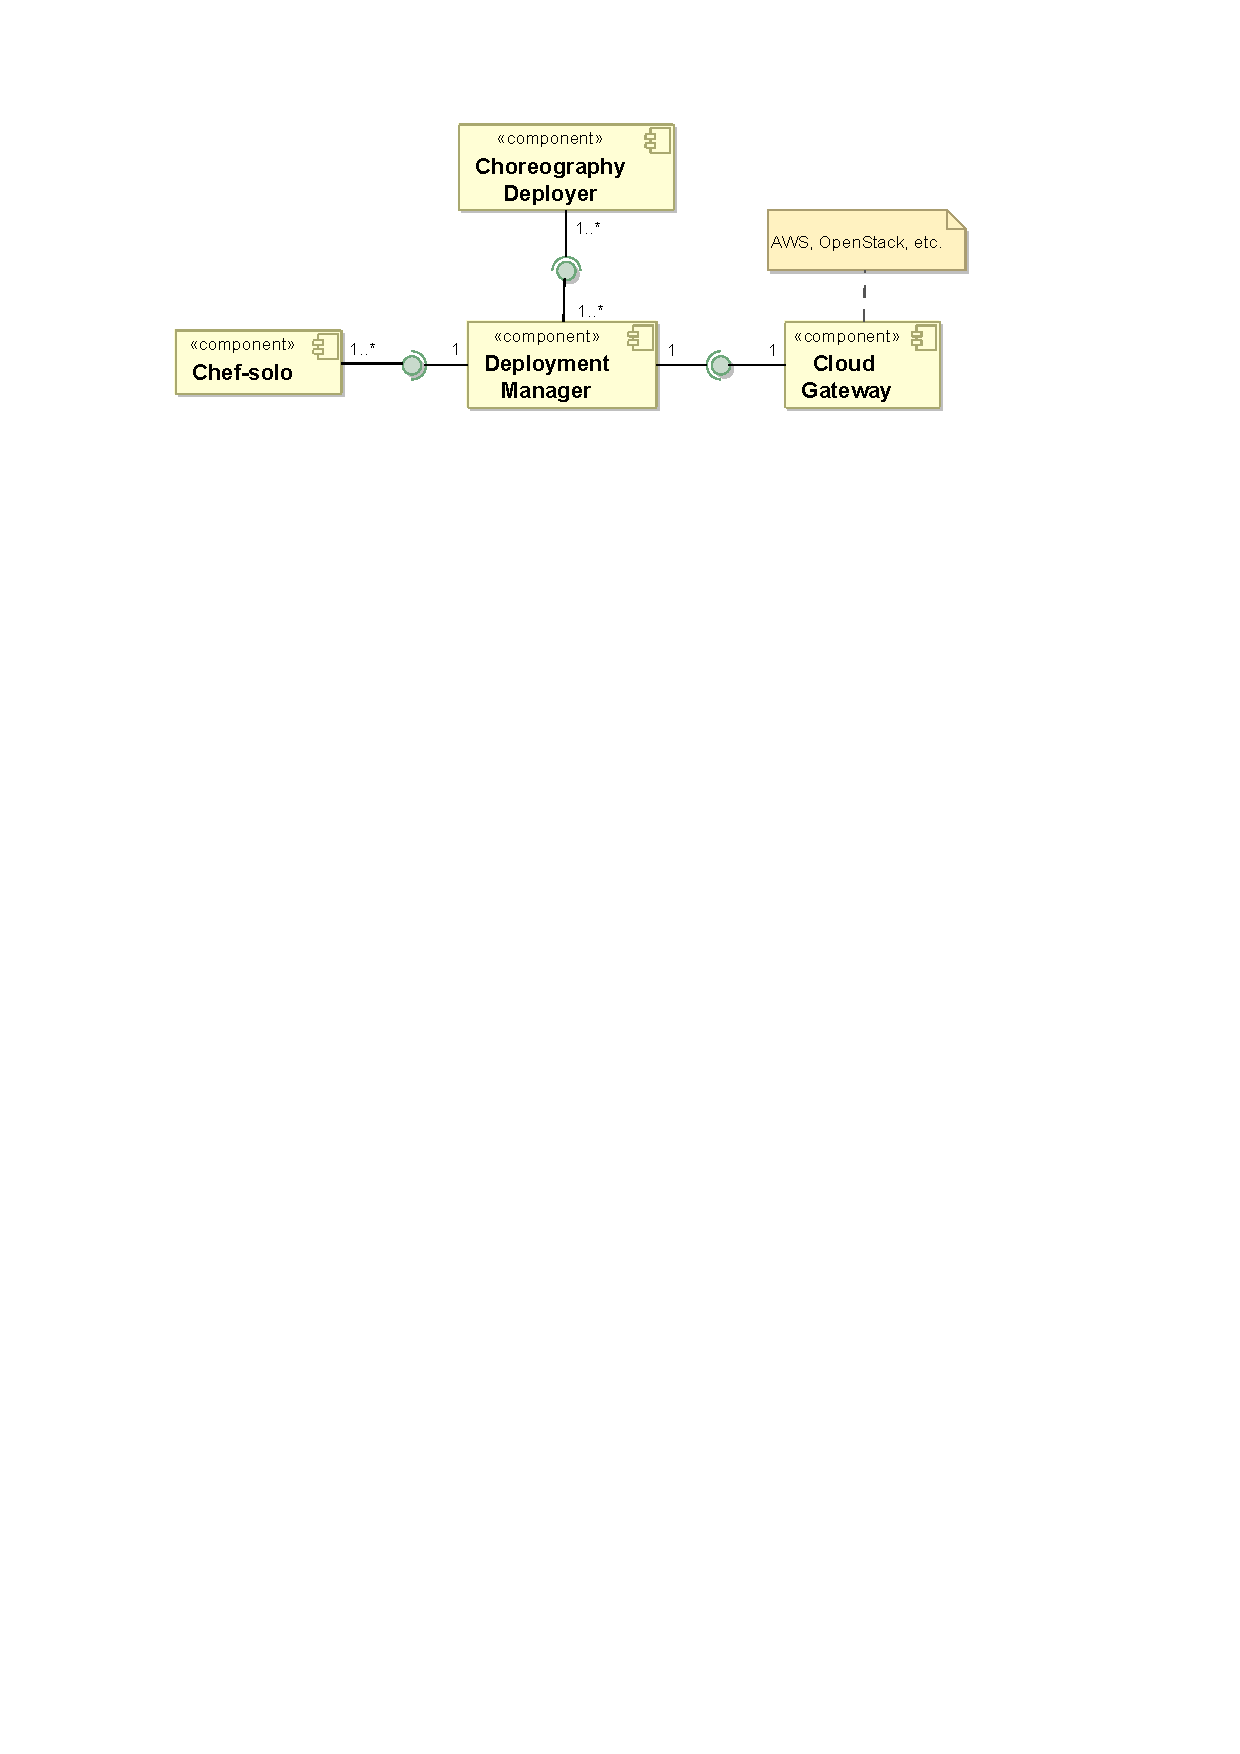
\includegraphics[scale=0.8]{img/components.pdf}
\caption{\ee\ architecture}
\label{fig:ee_components}
\end{figure}

\begin{description}

\item [Cloud Gateway] creates and destroys virtual machines (also called \emph{nodes}) in a cloud computing environment. This component is used by the \dm, that decides when to create or to destroy the nodes. Currently, only Amazon EC2 and OpenStack are supported as Cloud Gateways, but the \dm\ may be extended to support other virtualization technologies.

\item[Chef-solo] is installed by the \ee\ in each cloud node to manage ``recipes'' execution. \emph{Chef recipes} are scripts written in a Ruby-like Domain Specific Language that implement the process of configuring operational system, installing required middleware, and finally deploying the services.

\item [\dm] deploys services in a cloud environment. Through its REST API, the \dm\ receives a declarative service specification and selects the node where the service will be deployed, possibly considering the service non-functional requirements. The \dm\ executes in the selected node a process to generate the service recipe based on the service specification. Using other \dm\ REST operation, one can request the upgrade of a node, which consists in running Chef-solo on that node.

\item [\cd] exposes the REST API to web service choreography automated deployment. The \cd\ client must provide a choreography declarative specification, that contains the choreography architectural description and the locations of service packages. Based on this specification, the \cd\ coordinates invocations to the multiple \dm{s} belonging to the different participant organizations. After services deployment, the \cd\ provides the provider services locations to their respective consumer services.

\end{description} 

In this guide we assume that both \cd\ and \dm\ components will be executed on the deployer machine. Deployer is the human operator responsible by the deployment process. 

\section{Requirements}

Before you run \ee, you will need:

\begin{itemize}
\item SVN;
\item Java 6 or later (we are using OpenJDK);
\item Maven 3  (\url{http://maven.apache.org/download.html});
\item a Cloud Gateway access, as detailed in Section~\ref{sec:cloud}.
\end{itemize}

\section{Cloud Provider}
\label{sec:cloud}

A \textsf{CloudProvider} is an \ee\ interface that specifies methods to CRUD virtual machines. It is expected that a \textsf{Cloud Provider} implementations will act just as a client of some Cloud Gateway. In this section we describe the currently available \textsf{CloudProvider} implementations and how to use them. New \textsf{CloudProvider}s may be implemented to support other virtualization tools. One example would be creating a \textsf{VirtualBoxCloudProvider} to create VMs using VirtualBox.

Whatever the cloud provider you choose, ensure that the required TCP ports of the created VMs are unblocked. Required ports: 22 to SSH, 8080, 8009, and 8005 to Tomcat, the ports used by your JAR services, and the port 8180 to EasyESB.

\subsection{Amazon EC2}

Amazon EC2 service is the simplest choice to dynamically retrieve VMs as you need. You need just to create an account at \url{http://aws.amazon.com} and configure a pair of keys to access the VMs through SSH. The trade-off is that you must pay to Amazon! 

Some hints:

\begin{itemize}
\item Request credits to education purposes: \url{http://aws.amazon.com/grants/}. The first of us earned \$500, but the others \$100. Maybe it depends on your research project description.
\item Initially there is a limit of 20 VMs that you can run simultaneously.
\item Request to increase Amazon EC2 instance limit: \url{http://aws.amazon.com/contact-us/ec2-request/}. At USP we got a 50 VMs limit.
\item If you are going to use the EC2 API directly, pay attention to the ``one-second rule'': \\ \url{http://www.a2sdeveloper.com/page-working-with-the-one-second-rule.html}. Nonetheless, \ee\ already implements this rule.
\item As you will be charged per hour, don't forget to shutdown/stop unused VMs.
\item You can use the Amazon EC2 web console to unblock TCP ports necessary to the choreography execution.
\item You can also use the \texttt{ec2} command line tools to manage your VMs.
\item The \ee\ creates VMs in the ``US East'' Amazon datacenter.
\item The SSH keypairs are datacenter-dependent. Therefore if you create a keypair in the EU
datacenter, it won't be valid for your VMs.
\end{itemize}

\subsection{OpenStack}

OpenStack is an open source private cloud platform that provides services to retrieve VMs as you need, in the same way that Amazon EC2. However, you must install OpenStack in your own infrastructure, which means you must own at least a little cluster (or a very powerful machine) to host the created VMs. Moreover, the OpenStack installation and configuration is not a simple task.

Some hints:

\begin{itemize}
\item OpenStack does not provide public IPs, therefore some VPN configuration is necessary to log into the provisioned nodes.
\item you can also use the \texttt{nova} command line tool to manage your VMs.
\item you need to host an Ubuntu Server 12.04 image within your OpenStack infrastructure. You will use the ID of this image to configure \ee.
\end{itemize}

\subsection{Fixed cloud provider}

If you are learning how to use the \ee\ and want just to experiment it, the \textsf{FixedCloudProvider} may be the most suitable option to you. 
It is also useful if you want to use \ee\ with your own already existing cluster machines.
With it you are responsible to manually crating and setting virtual machines and telling to \ee\ which machines must be used by it. This avoids the overhead of dealing with a cloud environment. 

When creating a virtual machine to be used by the \ee, be sure:
\begin{itemize}
\item to use the Ubuntu 12.04 as operating system;
\item it is possible to SSH into the node without typing a password: \url{http://www.integrade.org.br/ssh-without-password}\footnote{Obs: do not use a key with password.};
\item use sudo in the machine without typing a password: type \texttt{\$sudo visudo} and add the line \texttt{<user> ALL = NOPASSWD: ALL} at the end (change \texttt{<user>} by the actual user);
\item to synchronize the machine clock: \texttt{\#ntpdate ccsl.ime.usp.br};
\end{itemize}

Configure the \texttt{deployment.properties} file settings, according to the template, to indicate which machines will be used by \ee.

To verify if your VM was properly set, you may run the \\ \textsf{org.ow2.choreos.deployment.nodes.cloudprovider.FixedConnectionTest} test.

The \ee\ \emph{will not} take care of bootstrapping (installing Chef) on your machines, since this process is taken only when creating new machines. 
You \emph{must} bootstrap your machines by running the \textsf{org.ow2.choreos.deployment.nodes.cm.BootstrapFixedMachines} class.

Depending on how you create your VMs, some network configuration may be needed. In case of using VirtualBox, you can refer to \url{http://ccsl.ime.usp.br/foswiki/bin/view/Choreos/VMs}.

\section{EasyESB}

The \ee\ enables the usage of a Distributed Service Bus, EasyESB~\footnote{\url{https://research.petalslink.org/display/easyesb}}, to bind the services according to the choreography specification. In this way, a service is not directly consumed by other services, but rather accessed through the bus. We also say that a service is ``proxified'' by the bus. The usage of the bus also enables some management and monitoring facilities. To enable the bus usage by \ee, add `\texttt{BUS=True}' to the \texttt{chordeployer.properties} configuration file. If this property is not set, the \ee\ deploys the services and bind them directly, without using the bus. If `\texttt{BUS=True}' is set, you must still set the \texttt{BUS\_POLICY} property on the same file. Possible values to the \texttt{BUS\_POLICY} property are:

\begin{description}
\item [SINGLE\_NODE:] \ee\ creates only a single EasyESB node, and all the deployed services are exposed by this esb node.
\item [ALWAYS\_CREATE:] each deployed service has a different associated EasyESB node. 
\item [LIMITED\_ROUND\_ROBIN:] initially new ESB nodes are created as in the ALWAYS\_CREATE policy. After a limit is reached, new proxifications are distributed to the existing ESB nodes in a round robin sequence. The limit is defined by the ESB\_NODES\_LIMIT property on \texttt{chordeployed.properties}
\end{description}

Obs: \ee\ always create a new cloud node to host each EasyESB node.

\section{Checkout and Compilation}

To checkout the code: \texttt{svn checkout svn://svn.forge.objectweb.org/svnroot/choreos/trunk/cloud cloud}. 

After installing Maven 3, open the terminal at the \texttt{choreos\_middleware} folder, and run the \texttt{build.sh} script. It can take several minutes. Internet access is necessary during compilation.

\section{Configuration}

Open the folder \texttt{DeploymentManager/src/main/resources}, and create a \texttt{deployment.properties} file by copying the \texttt{deployment.properties.template} file. The new properties file must be created in the same folder. Open the just created properties file and edit it following instructions on the template file. The Listing~\ref{lst:deployment_properties} shows an example. Do the same process to the template properties file \texttt{ChoreographyDeployer/src/main/resources/deployment.properties}.

\lstset{
numbers=left
}

{\footnotesize
\begin{lstlisting}[caption=deployment.properties example,label=lst:deployment_properties] 
DEPLOYMENT_MANAGER_PORT=9100
CLOUD_PROVIDER=AWS
NODE_SELECTOR=LIMITED_ROUND_ROBIN
VM_LIMIT=5

FIXED_VM_IPS=192.168.56.101
FIXED_VM_HOSTNAMES=leo-arch-node
FIXED_VM_PRIVATE_SSH_KEYS=/home/leonardo/.ssh/nopass
FIXED_VM_USERS=choreos
MAPPER_POLICY=ANY_FIT
FIXED_VM_TYPES=SMALL

AMAZON_ACCESS_KEY_ID=SECRET
AMAZON_SECRET_KEY=SECRET
AMAZON_KEY_PAIR=leoflaws
AMAZON_PRIVATE_SSH_KEY=/home/leonardo/.ssh/leoflaws.pem
AMAZON_IMAGE_ID=us-east-1/ami-1ccc8875

OPENSTACK_KEY_PAIR=leofl
OPENSTACK_PRIVATE_SSH_KEY=/home/leonardo/.ssh/nopass
OPENSTACK_TENANT=CHOReOS_Sandbox
OPENSTACK_USER=leofl
OPENSTACK_PASSWORD=SECRET
OPENSTACK_IP=http://172.15.237.10:5000/v2.0
OPENSTACK_IMAGE_ID=RegionOne/1654b5b6-49b7-4039-b7b7-0e42e85480f4

IDLE_POOL_SIZE=0

\end{lstlisting}
}

Options to CLOUD\_PROVIDER: AWS, OPEN\_STACK, and FIXED.

The options to NODE\_SELECTOR are: 

\begin{description}
\item [ALWAYS\_CREATE:] a new VM is created to each deployed service instance;
\item [ROUND\_ROBIN:] \textsf{NodeSelector} makes a round robin using the available VMs, without creating any new VM;
\item [LIMITED\_ROUND\_ROBIN:] initially the \textsf{NodeSelector} behaves like the ALWAYS\_CREATE, until a limit of created VMs is reached (VM\_LIMIT). After this limit, the selector behaves like the ROUND\_ROBIN. When using this selector, it is necessary to declare the integer VM\_LIMIT property in the configuration file.
\end{description}

The IDLE\_POOL\_SIZE makes the Deployment Manager operate with a pool of idle nodes, which makes the node retrieval to be faster when some IaaS fault occurs. The use of this pool makes the deployment process more scalable, however the trade-off is the cost of some more VMs created by the infrastructure provider. 

The AMAZON\_IMAGE\_ID enables you to specify a customized image to be used by \ee. This feature is intended to use an image of a node already bootstrapped. In this way, the bootstrap process becomes much faster. The same may be applied to the OPENSTACK\_IMAGE\_ID. But in both cases, the image must still provide an Ubuntu Server 12.04 system.

Other options are explained in the \texttt{deployment.properties.template} file.

In the \texttt{ChoreographyDeployer} project you may also edit the file \texttt{owners.properties}. If you are going to use only one cloud infrastructure, and the default \ee\ configuration\footnote{Choreography Deployer and Deployment Manager on the same machine, and both using their respective default ports.}, the file do not need to be changed. If you are going to use multiple cloud environments, you need to configure one Deployment Manager to each cloud infrastructure. So, you must configure the \texttt{owners.properties} file to give a name to each available Deployment Manager. These names will be compared with the \texttt{owner} attribute in the  service specifications, so the service can be deployed by the matched Deployment Manager. If there is no match, the DEFAULT value declared on \texttt{owners.properties} will be used.

\emph{Attention:} inline comments are not allowed in properties files. Therefore, the following would not work: \verb!VM\_LIMIT=3 \# how many instances we can afford to pay!

\section{Execution}

After compiling the project, to run both \cd\ and \dm\ you have just to run the main method on the following classes: \textsf{org.ow2.choreos.deployment.rest.DeploymentManagerServer} and \textsf{org.ow2.choreos.chors.rest.ChorDeployerServer}.

This task can be easier accomplished if you import the \ee\ projects in the Eclipse IDE. After importing the project, open the menu \texttt{Window>>Preferences>>Java>>Build Path>>Classpath} variables, and set the \texttt{M2\_REPO} variable pointing to your Maven repository folder, usually the \texttt{.m2/repository} folder within your home folder. Obs: we have used the Eclipse Indigo version.

Another way is using maven:

\texttt{DeploymentManager\$ mvn exec:java}

\texttt{ChoreographyDeployer\$ mvn exec:java}

If you successfully start the \cd\ and the \dm\, you must see the following messages on their respective consoles: 

\texttt{\cd\ has started [http://localhost:9100/choreographydeployer/]}

\texttt{\dm\ has started [http://localhost:9101/deploymentmanager/]}

To verify if it is everything OK, run the \textsf{org.ow2.choreos.chors.SimpleChorEnactmentTest}. This test will deploy a simple choreography composed of two services and try to invoke it.
